\documentclass[a4paper]{article}
\usepackage{amsmath}
\addtolength{\hoffset}{-2.25cm}
\addtolength{\textwidth}{4.5cm}
\addtolength{\voffset}{-3.25cm}
\addtolength{\textheight}{5cm}
\setlength{\parindent}{15pt}

\usepackage[unicode=true, colorlinks=false, hidelinks]{hyperref}
\usepackage[utf8]{inputenc}
\usepackage[english, russian]{babel}
\usepackage{mathtext}
\usepackage[T2A, TS1]{fontenc}
\usepackage{microtype} % Slightly tweak font spacing for aesthetics
\usepackage{amsthm, amssymb, amsmath, amsfonts, nccmath}
\usepackage{nicefrac}
\usepackage{epstopdf}
\usepackage[export]{adjustbox}
\usepackage{float} % Improved interface for floating objects
\usepackage{graphicx, multicol} % Enhanced support for graphics
\usepackage{pdfrender,xcolor}
\usepackage{breqn}
\usepackage{mathtools}
\usepackage{titling}
\usepackage{bm}
\usepackage{centernot}
\usepackage[cal=boondoxo,calscaled=.96]{mathalpha}
\usepackage{marvosym, wasysym} % More symbols
\usepackage{rotating} % Rotation tools
\usepackage{censor} % Facilities for controlling restricted text

\usepackage{fancyhdr}
\pagestyle{fancy}
\fancyhead{}\renewcommand{\headrulewidth}{0pt}
\fancyfoot[L]{}
\fancyhead{}
\fancyfoot{}
\fancyfoot[R]{\thepage}
\begin{document}
    \begin{titlepage}
   \begin{center}
       \vspace*{3cm}
       \large{САНКТ-ПЕТЕРБУРГСКИЙ ПОЛИТЕХНИЧЕСКИЙ УНИВЕРСИТЕТ}
       \vspace{0.4 cm}

       \large\textbf{Институт прикладной математики и механики}
       \vspace{0.4 cm}

       \large{Высшая школа прикладной математики и вычислительной физики}

       \vspace{3 cm}
       \normalsize\textbf{Отчет\\ по лабораторной работе №7\\ по дисциплине\\
«Математическая статистика»}
       \vfill
       \begin{flushright}
            \normalsize{Выполнил студент:\\
            Антонов Алексей\\
            группа: 3630102/80201}
            \vskip\medskipamount
            \normalsize{Проверил:

            к.ф.-м.н., доцент\\
            Баженов Александр Николаевич
            }
       \end{flushright}

       \vspace{0.8cm}


       \normalsize{Санкт-Петербург\\2021 г.}

   \end{center}
\end{titlepage}
    \tableofcontents
    \newpage
    \listoftables
    \newpage
\section {Постановка задачи}
\noindent Для 5 распределений:
\begin{enumerate}
	\item $N(x, 0, 1)$ -- нормальное распределение
	\item $C(x, 0, 1)$ -- распределение Коши
	\item $L(x, 0, \frac{1}{\sqrt{2}})$ -- распределение Лапласа
	\item $P(k, 10)$ -- распределение Пуассона
	\item $U(x, -\sqrt{3}, \sqrt{3})$ -- расномерное распределение
\end{enumerate}
Сгенерировать выборки размером 20 и 100 элементов.
Построить для них боксплот Тьюки.
Для каждого распределения определить долю выбросов экспериментально (сгенерировав выборку, соответствующую распределению 1000 раз, и вычислив среднюю долю выбросов) и сравнить с результатами, полученными теоретически.


\section {Теория}
\subsection{Боксплот Тьюки}
	\subsubsection{Определение}
	\noindent Боксплот (англ. box plot) — график, использующийся в описательной статистике, компактно изображающий одномерное распределение вероятностей

	\subsubsection{Описание}
	\noindent Такой вид диаграммы в удобной форме показывает медиану, нижний и верхний квартили и выбросы. Несколько таких ящиков можно нарисовать бок о бок, чтобы визуально сравнивать одно распределение с другим; их можно располагать как горизонтально, так и вертикально. Расстояния между различными частями ящика позволяют определить степень разброса (дисперсии) и асимметрии данных и выявить выбросы.

	\subsubsection{Построение}
	\noindent Границами ящика служат первый и третий квартили, линия в середине ящика — медиана. Концы усов — края статистически значимой выборки (без выбросов). Длину «усов» определяют разность первого квартиля и полутора межквартильных расстояний и сумма третьего квартиля и полутора межквартильных расстояний. Формула имеет вид
	\begin{equation}
	\label{mouns}
	{X_1 = Q_1-} \frac{3}{2}{(Q_3 - Q_1)},   {X_2 = Q_3+} \frac{3}{2}{(Q_3 - Q_1)}
	\end{equation}
	где $X_1$ — нижняя граница уса, $X_2$ — верхняя граница уса, $Q_1$ — первый квартиль, $Q_3$ — третий квартиль. Данные, выходящие за границы усов (выбросы), отображаются на графике в виде маленьких кружков.


\subsection{Теоретическая вероятность выбросов}
	\noindent Встроенными средствами языка программирования Python в среде разработки PyCharm можно вычислить теоретические первый и третий квартили распределений ($Q_1^T$ и $Q_3^T$ соответственно). По формуле \eqref{mouns} можно вычислить теоретические нижнюю и верхнюю границы уса ($X_1^T$ и $X_2^T$ соответственно). Выбросами считаются величины x, такие что:
	\begin{equation}
		\left[
		\begin{gathered}
		x < X_1^T \\
		x > X_2^T \\
		\end{gathered}
		\right.
	\end{equation}
	Теоретическая вероятность выбросов для непрерывных распределений
	\begin{equation}
		P_B^T = P(x<X_1^T) + P(x>X_2^T)=F(X_1^T) + (1-F(X_2^T))
	\end{equation}
	где $F(X)=P(x\leq{X})$ - функция распределения.
	Теоретическая вероятность выбросов для дискретных распределений
	\begin{equation}
		P_B^T = P(x<X_1^T)+P(x>x_2^T)=(F(X_1^T)-P(x=X_1^T))+(1-F(X_2^T))
	\end{equation}
	где $F(X) = P(x\leq{X})$ - функция распределения

\section{Программная реализация}
Лабораторная работа выполнена на языке Python в среде PyCharm с использованием следующих библиотек:
\begin{enumerate}
    \item numpy
    \item scipy
    \item matplotlib
\end{enumerate}

\section {Результаты}
\subsection{Боксплот Тьюки}
\begin{figure}[H]
\center{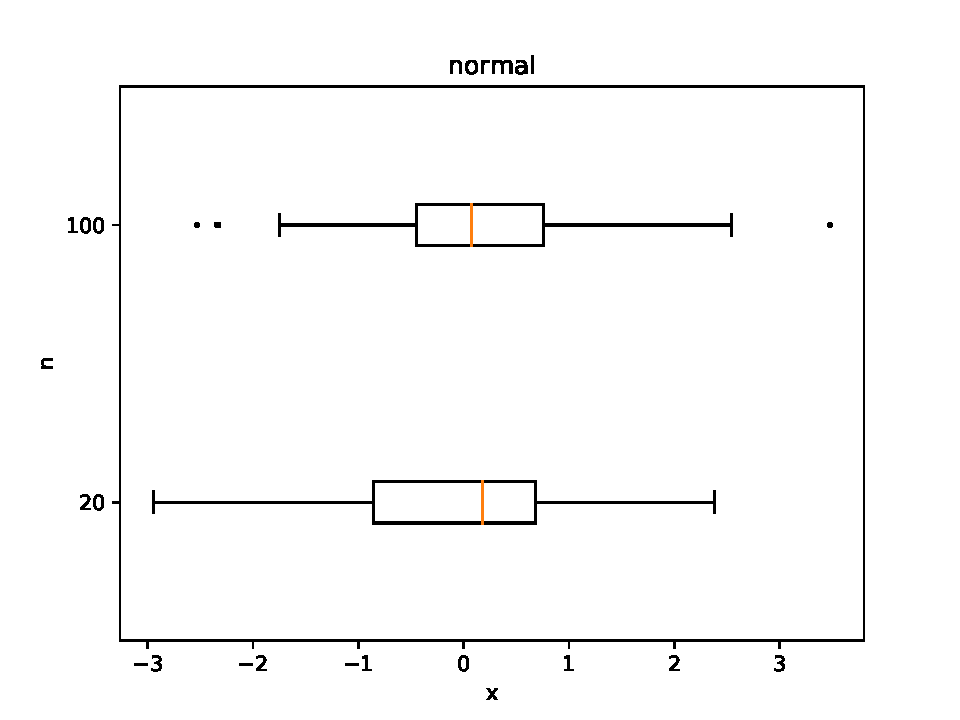
\includegraphics[scale=0.75]{src/normal}}
\label{fig:normal}
\caption{Нормальное распределение}
\end{figure}

\begin{figure}[H]
\center{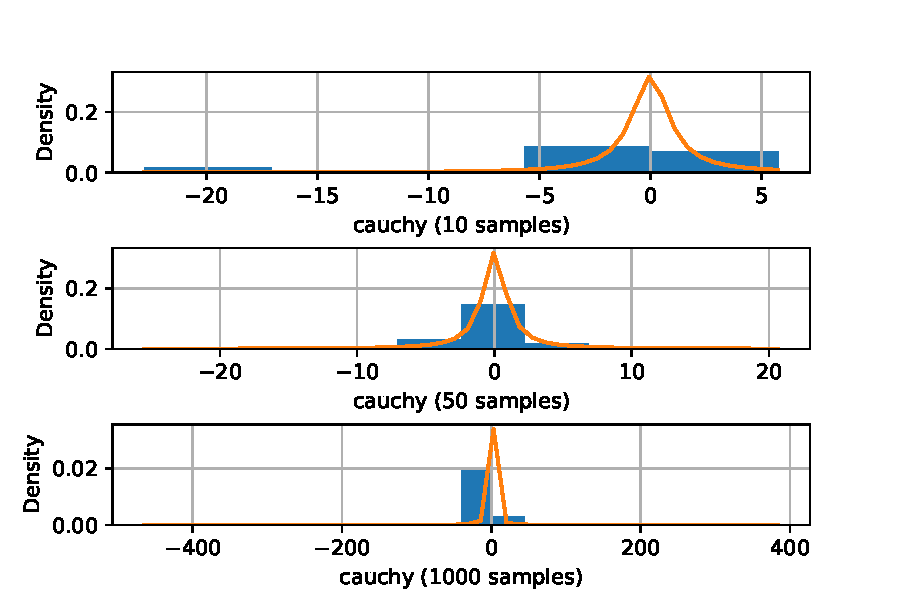
\includegraphics[scale=0.75]{src/cauchy}}
\label{fig:cauchy}
\caption{распределение Коши}
\end{figure}

\begin{figure}[H]
\center{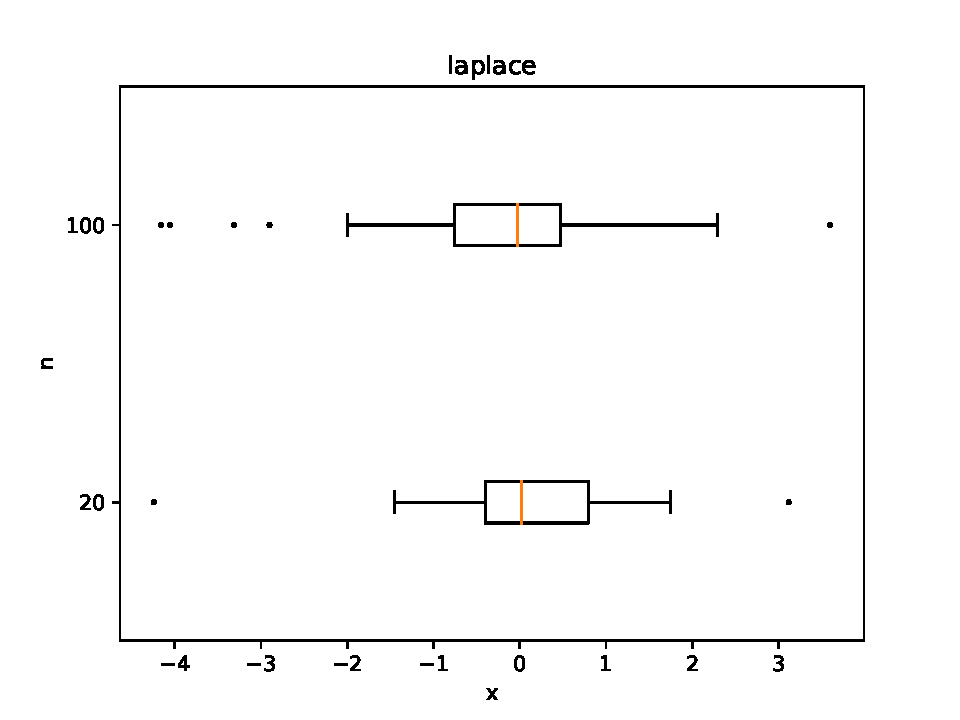
\includegraphics[scale=0.75]{src/laplace}}
\label{fig:laplace}
\caption{распределение Лапласа}
\end{figure}

\begin{figure}[H]
\center{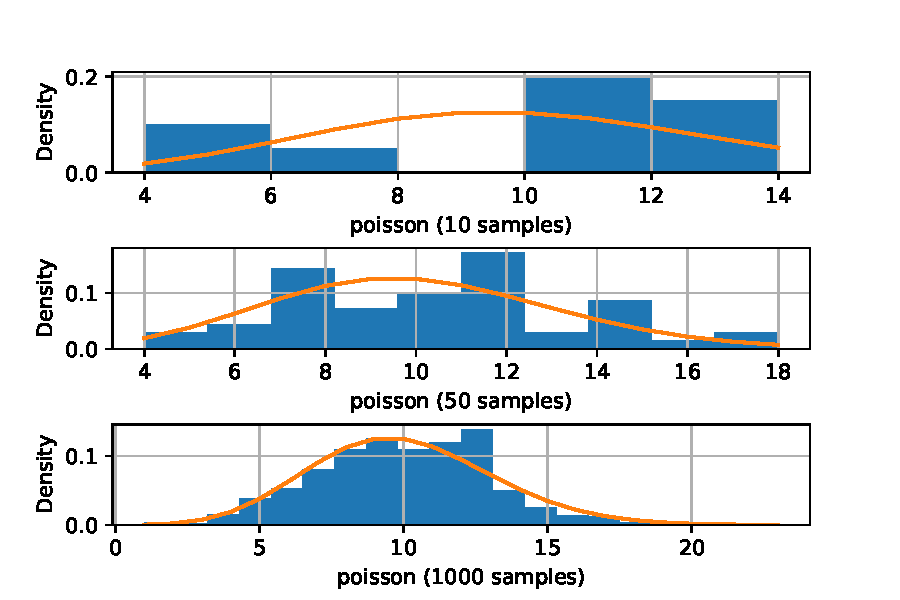
\includegraphics[scale=0.75]{src/poisson}}
\label{fig:poisson}
\caption{распределение Пуассона}
\end{figure}

\begin{figure}[H]
\center{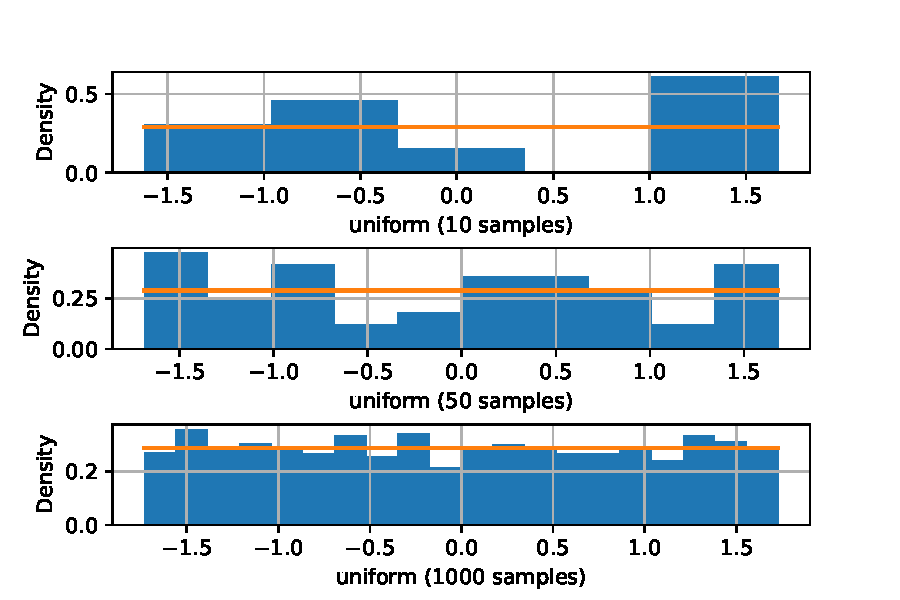
\includegraphics[scale=0.75]{src/uniform}}
\label{fig:uniform}
\caption{равномерное распределение}
\end{figure}

\subsection{Доля выбросов}
\begin{table}[H]
            \centering
            \begin{tabular}{|c|c|c|}
                \hline
                sample size&20&100\\ \hline
normal&0.024&0.01\\ \hline
cauchy&0.155&0.157\\ \hline
laplace&0.076&0.064\\ \hline
poisson&0.025&0.011\\ \hline
uniform&0.003&0.0\\ \hline

            \end{tabular}
            \caption{Доля выбросов}
            \label{tab:experimental_anomaly}
            \end{table}


\subsection{Теоретическая вероятность выбросов}
\begin{table}[H]
            \centering
            \begin{tabular}{|c|c|c|c|c|c|}
                \hline
                &$Q^{T}_{1}$&$Q^{T}_{3}$&$X^{T}_{1}$&$X^{T}_{2}$&$P^{T}_{B}$\\ \hline
normal&-0.674&0.674&-2.698&2.698&0.007\\ \hline
cauchy&-1.0&1.0&-4.0&4.0&0.156\\ \hline
laplace&-0.49&0.49&-1.961&1.961&0.062\\ \hline
poisson&8.0&12.0&2.0&18.0&0.008\\ \hline
uniform&-0.866&0.866&-3.464&3.464&0.0\\ \hline

            \end{tabular}
            \caption{Теоретическая вероятность выбросов}
            \label{tab:theoretical_anomaly}
            \end{table}

\section{Обсуждение}
В данной работе видно, что боксплоты Тьюки удобны для взуального представления важных
характеристик выборки. Из них можно делать выводы относительно
вида распределения, которому подчиняется выборка.

Данные в таблице говорят о том, что чем выше размер выборки, тем ближк доля выбросов к теоретической оценке. У распределения коши наблюдается самая высокая доля выбросов, в то время как в равномерном распределении доля выбросов близка к 0.

\section{Приложение}

\noindent Код программы GitHub URL:\\
\newline https://github.com/Brightest-Sunshine/Math-Statistic-2021/blob/main/Lab3/Lab3.ipynb

\end{document}

